Comparisons of tower energy spectra in transverse UE revealed an excess of events with an OHCal tower having an abnormally negative energy value in data relative to simulation. Figure~\ref{fig:UE_spectra_sim_vs_49219} shows the comparison of these spectra from a single Run 49219 in data to the 10 GeV Run 21 simulation. A total of 66 events were found in Run 49219 that contained an OHCal tower with E$_T <$ --3 GeV. These event numbers were collected and the waveforms of the OHCal towers were inspected for irregularities. Since the data was zero-suppressed, only the ADC values for time samples 0 and 6 were saved in the calorimeter DST files rather than the entire waveform. It was discovered that the waveforms of these towers had a large ADC at time sample 0 and an ADC consistent with pedestal levels at sample 6, where the signal would be expected. This could be consistent with the triggered event being in the adjacent bunch crossing immediately after a collision.

\begin{figure}
    \centering
    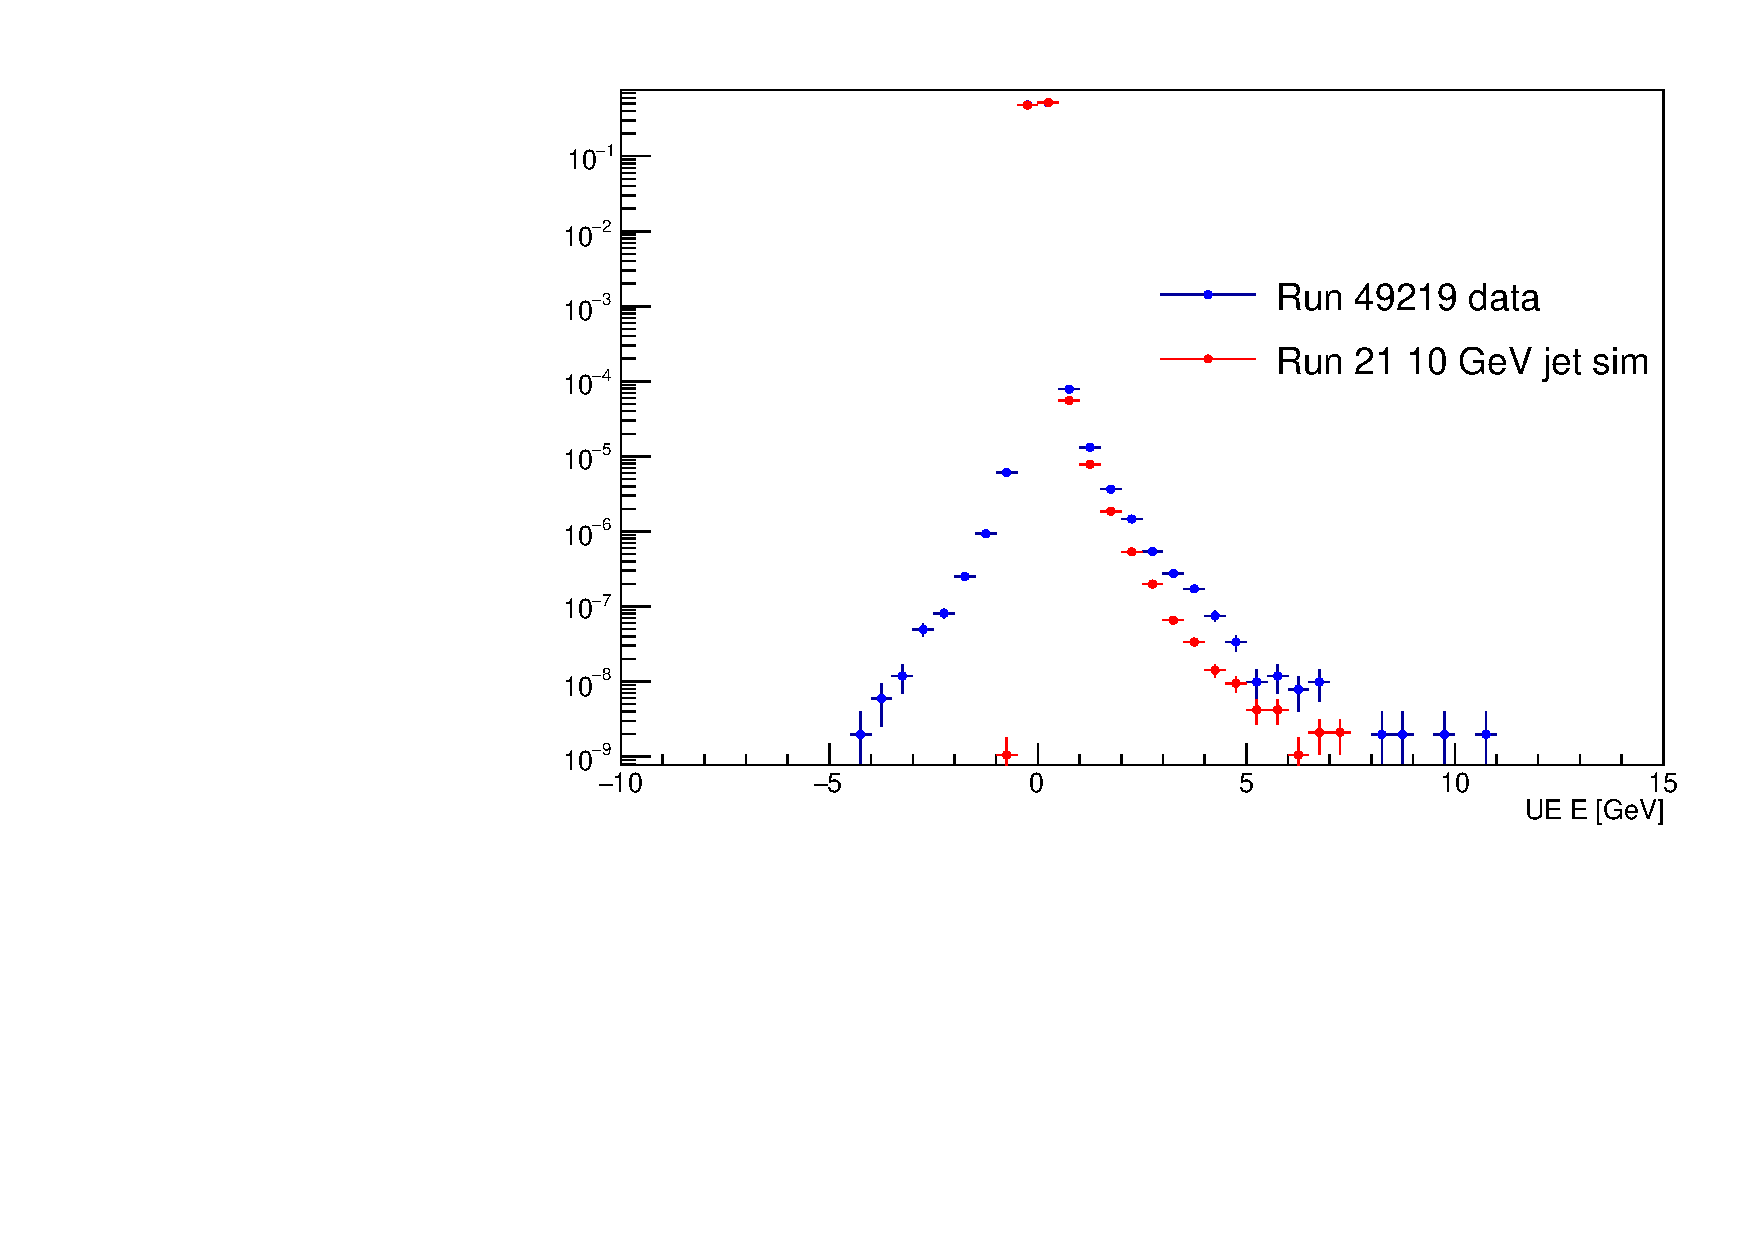
\includegraphics[width=0.5\linewidth]{Figures/mbd_waveforms_pileup/UE_spectra_sim_vs_49219.pdf}
    \caption{Transverse UE tower energy spectra for Run 49219 in data (blue) and Run 21 simulation (red).}
    \label{fig:UE_spectra_sim_vs_49219}
\end{figure}

To test if these very negative UE towers are in fact the result of out-of-time pileup, the MBD waveforms were plotted for 12 of the 66 events having an OHCal tower with energy below --3 GeV. A typical event will have an MBD waveform with a single peak around time sample 8, but an event with out-of-time pileup will contain more than one peak in its waveform. The MBD has 64 arms on each the North and South side, so all 128 waveforms were plotted together in a 2D histogram for simplicity. Fig.~\ref{fig:MBD_2D_waveforms} shows these waveforms and their corresponding event numbers. It is immediately apparent from these 2D waveforms that each of these 12 events were triggered on a bunch crossing directly after a crossing that contained a collision.

\begin{figure}
    \centering
    \begin{subfigure}{.329\textwidth}
    \centering
      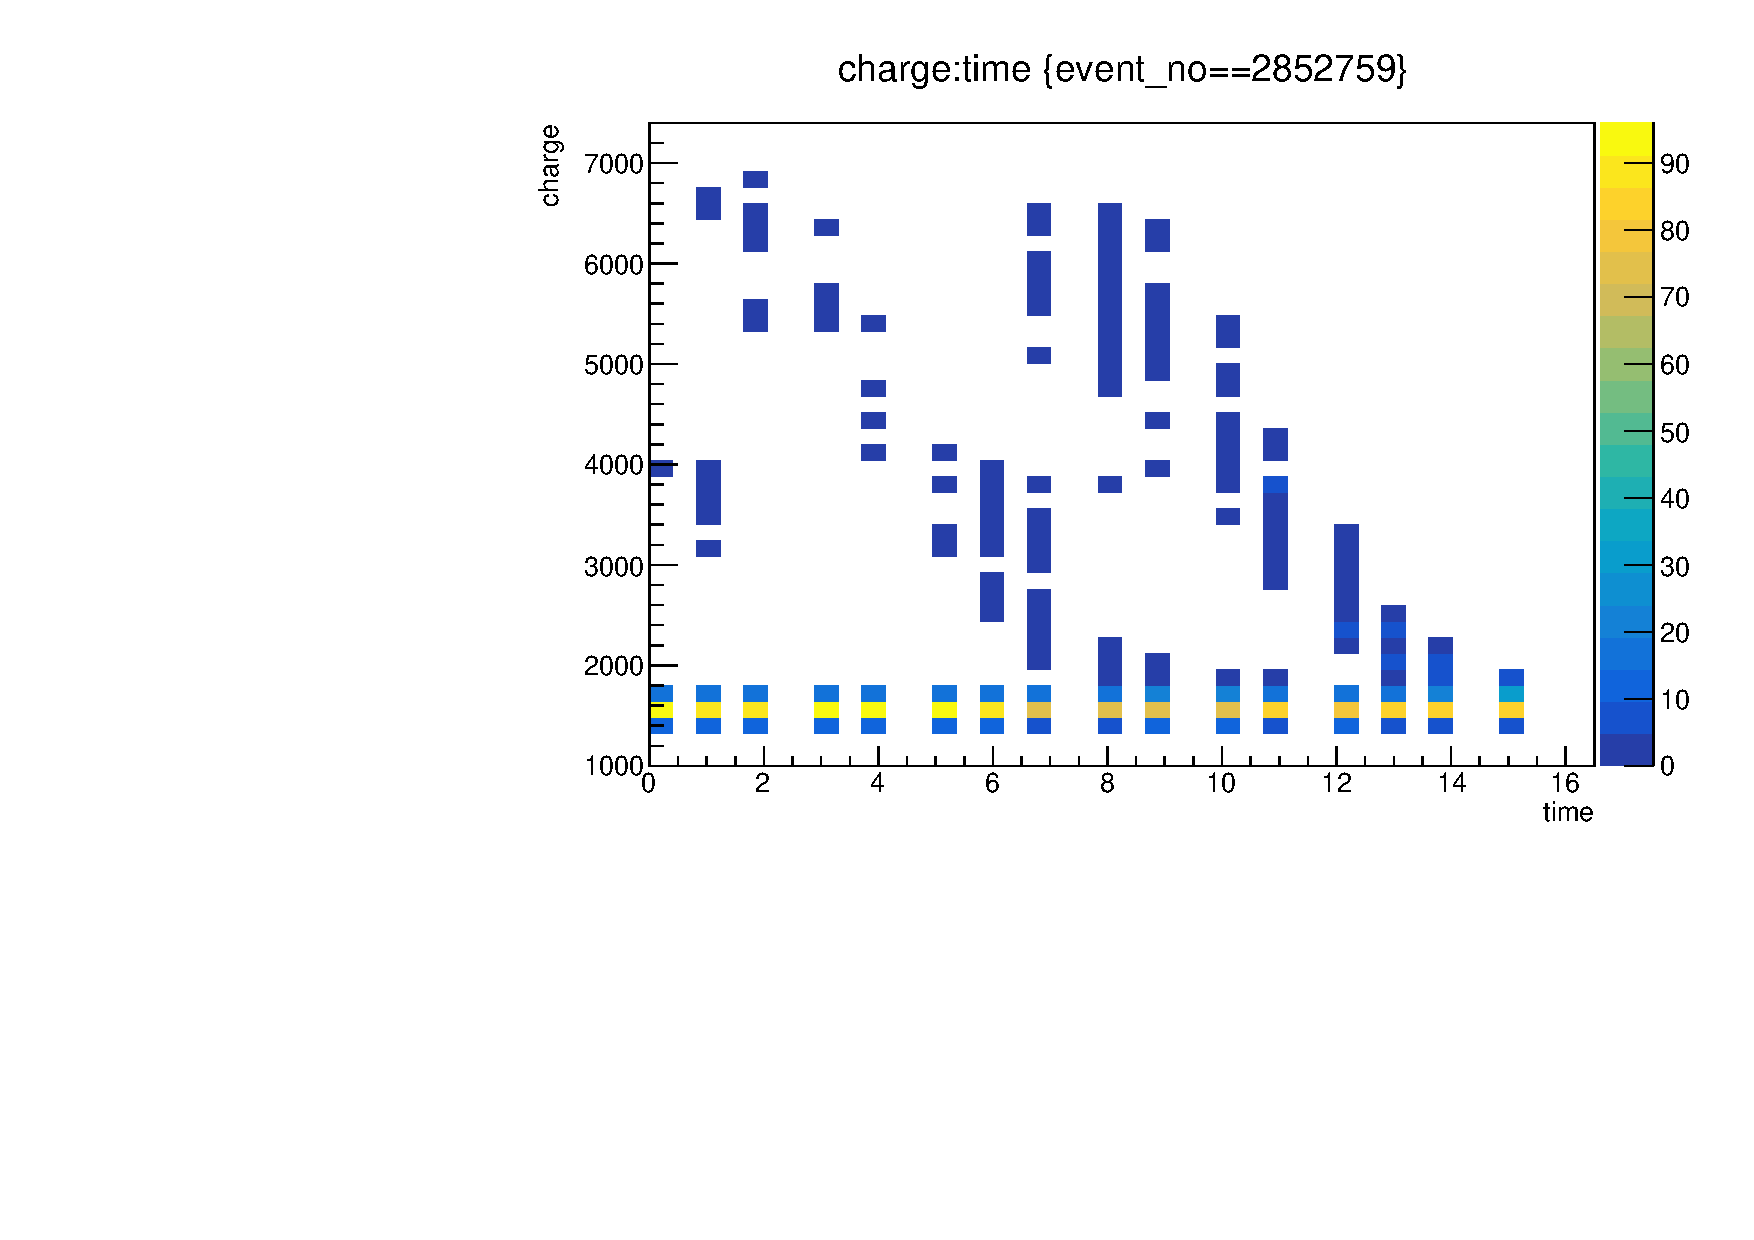
\includegraphics[width=1.\textwidth]{Figures/mbd_waveforms_pileup/MBD_2D_evt2852759.pdf}
    \end{subfigure}
    \begin{subfigure}{.329\textwidth}
    \centering
        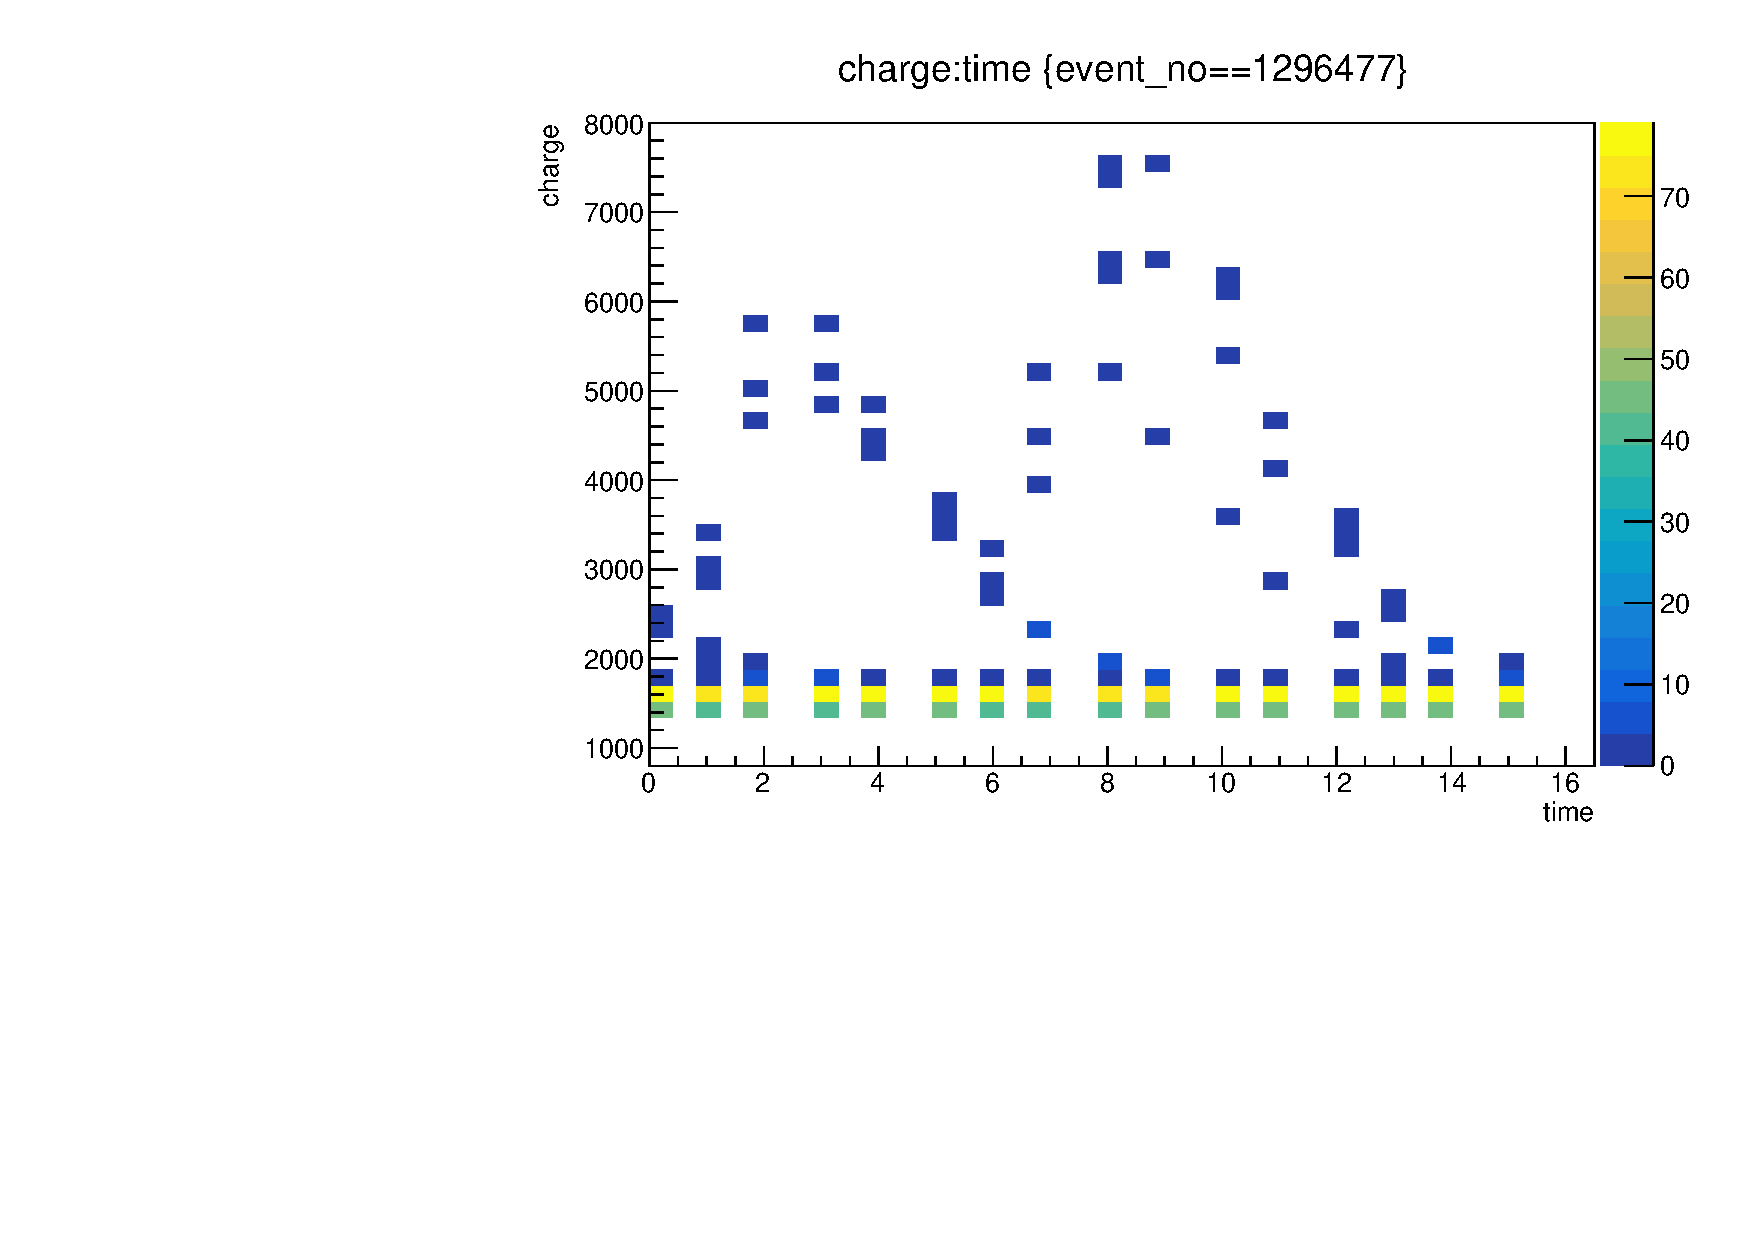
\includegraphics[width=1.\textwidth]{Figures/mbd_waveforms_pileup/MBD_2D_evt1296477.pdf}
    \end{subfigure}
    \begin{subfigure}{.329\textwidth}
    \centering
        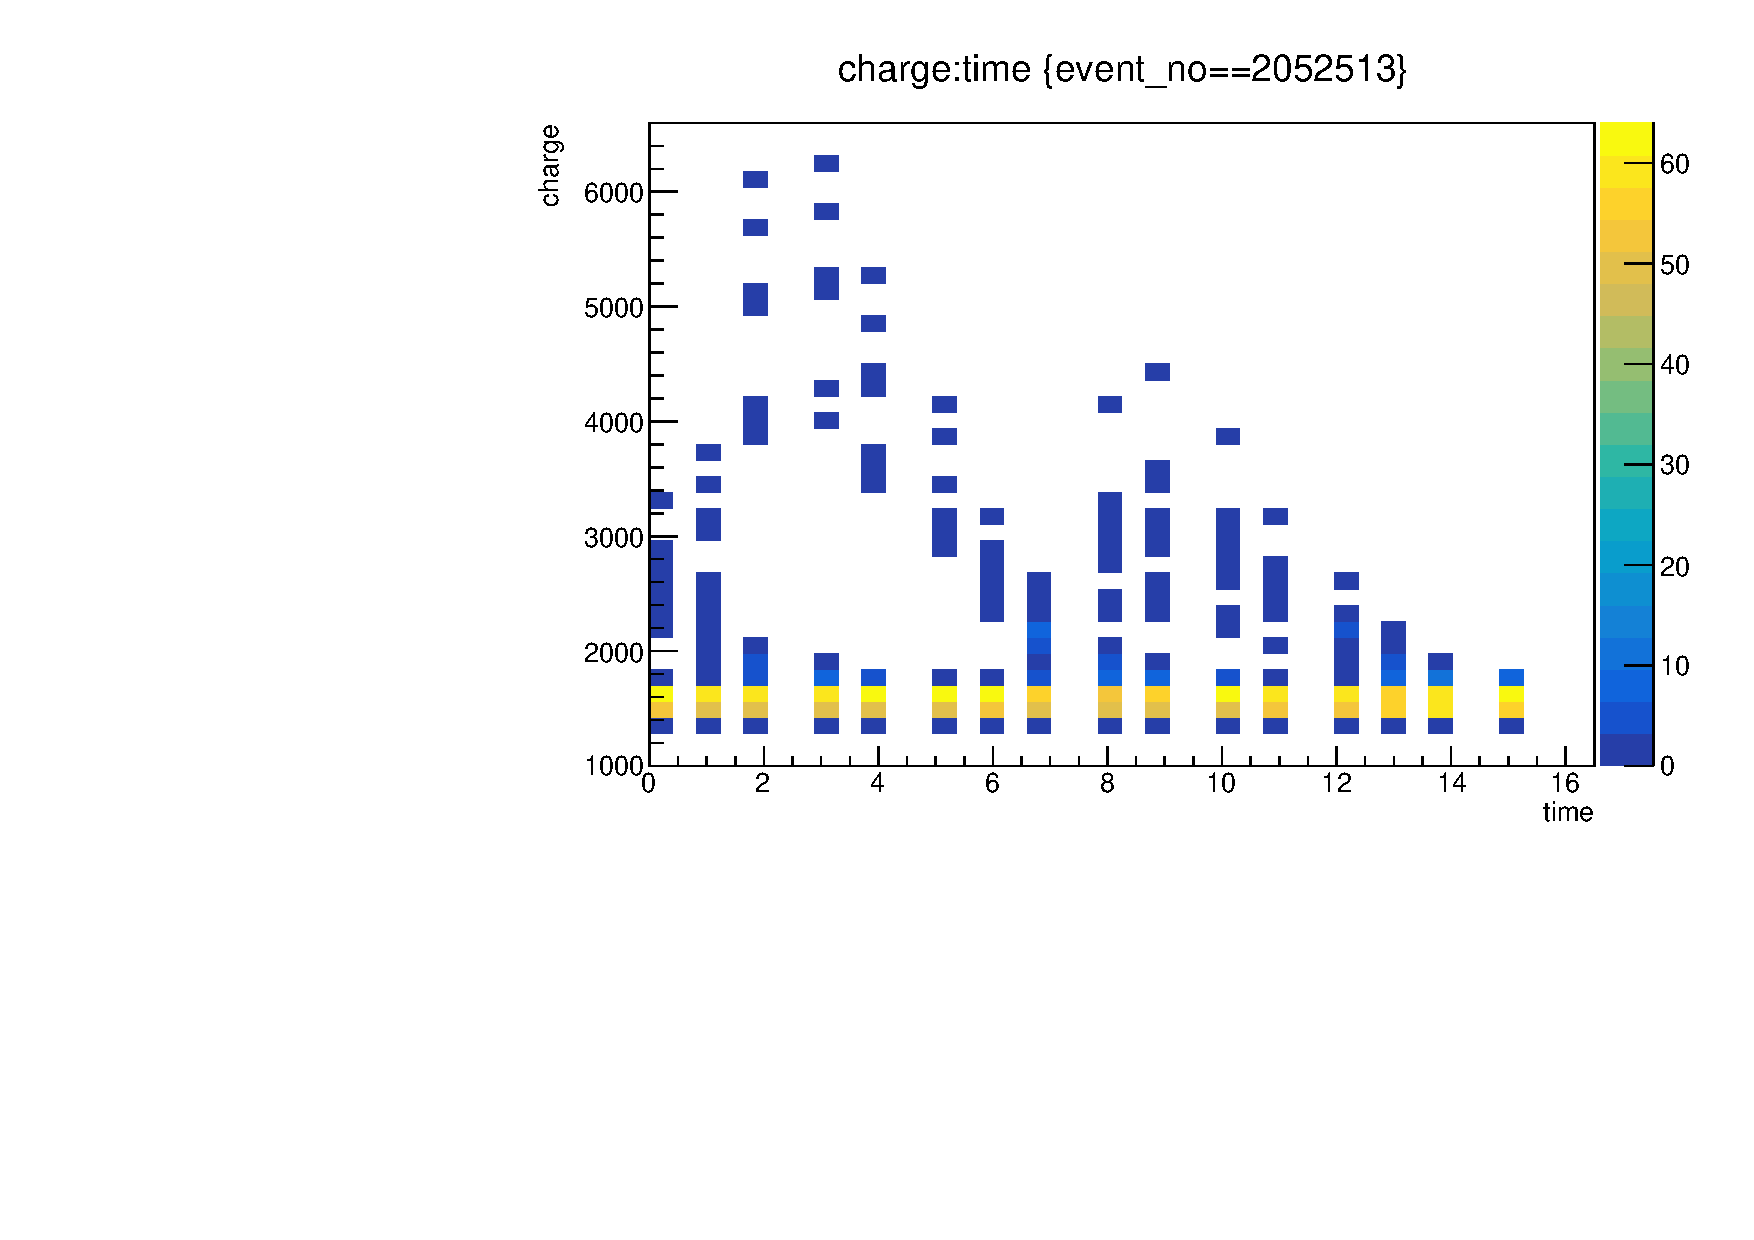
\includegraphics[width=1.\textwidth]{Figures/mbd_waveforms_pileup/MBD_2D_evt2052513.pdf}
    \end{subfigure}
    \caption{MBD waveform plots for 3 of the 66 events in run 49219 which contained an OHCal tower with energy below --3 GeV.}
\label{fig:MBD_2D_waveforms}
\end{figure}

%%  DISCUSS CORRECTION:
%%  - plot spectra for sum(E) > or < 0
%%  - determine E-value at which sum(E) < 0 spectra becomes dominant (~5x the positive sum(E) spectra) 
%%  - place min tower E-value
%%  - effect on observables (Emma???)